
\subsection{Data Efficiency of Hierarchical Knowledge Transfer}
\label{subsec:data-efficiency}

Figure~\ref{fig:cp-label-efficiency} presents the surface-pressure prediction errors of M0, M1, and M2 on 88 test wings under different target-domain training budgets. Both RMSE and MAE decrease with increasing training size, while the three knowledge configurations exhibit a consistent performance hierarchy. Incorporating sectional aerodynamic knowledge enables M1 to outperform the target-only baseline M0 across all training budgets. With the additional wing-root and wing-tip corrections, M2 further improves prediction accuracy. These results indicate that transferable sectional knowledge provides an effective basis for wing pressure prediction, while regional aerodynamic knowledge offers additional information for representing three-dimensional pressure variations.

\begin{figure*}[!t]
    \centering
    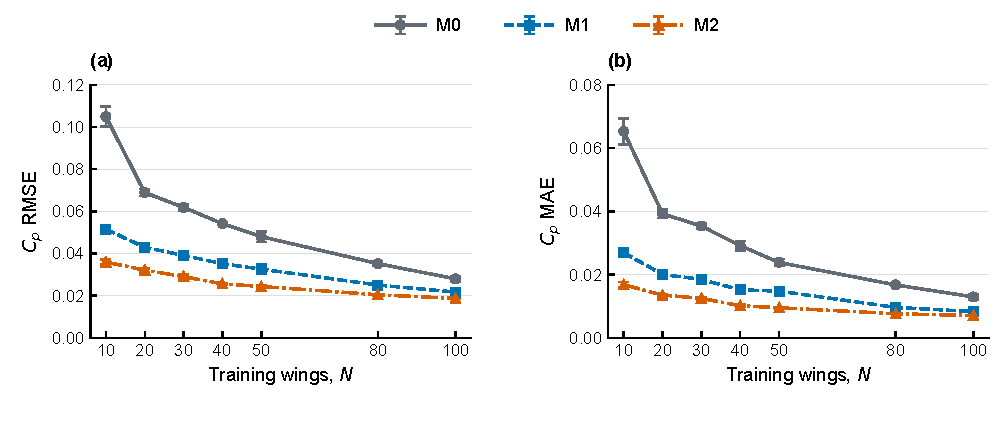
\includegraphics[width=0.90\textwidth]{V_Results_and_Discussion/figures/V_A_Fig13/V_A_Fig13_cp_label_efficiency.pdf}
    \caption{urface-pressure prediction errors at different training sizes: (a) RMSE and (b) MAE. Results are evaluated on 88 test wings over three runs.}
    \label{fig:cp-label-efficiency}
\end{figure*}


The benefit of hierarchical knowledge transfer is particularly evident under limited target-domain supervision. At $N=10$, M2 achieves an RMSE of 0.03593, corresponding to a mean reduction of 65.74\% relative to M0, as summarized in Table~\ref{tab:cp-data-efficiency}. Although the relative improvement from hierarchical knowledge transfer decreases as the target-domain training size increases, M2 consistently achieves the lowest prediction error across all training budgets. This indicates that sectional aerodynamic knowledge and regional corrections provide complementary information for target-domain pressure prediction across different data regimes, with particularly pronounced benefits when only limited target-domain samples are available.

\begin{table*}[!t]
    \centering
    \caption{Surface-pressure RMSE on 88 test wings at representative training sizes.}
    \label{tab:cp-data-efficiency}
    \small
    \renewcommand{\arraystretch}{1.15}
    \begin{tabular}{ccccc}
        \hline
        Training wings $N$ & M0 & M1 & M2 & M2 vs. M0 (\%) \\
        \hline
        10  & $0.10493 \pm 0.00470$ & $0.05150 \pm 0.00072$ & $0.03593 \pm 0.00117$ & 65.74 \\
        20  & $0.06893 \pm 0.00164$ & $0.04293 \pm 0.00094$ & $0.03210 \pm 0.00077$ & 53.43 \\
        50  & $0.04797 \pm 0.00250$ & $0.03258 \pm 0.00210$ & $0.02434 \pm 0.00079$ & 49.15 \\
        100 & $0.02796 \pm 0.00117$ & $0.02170 \pm 0.00157$ & $0.01869 \pm 0.00034$ & 33.04 \\
        \hline
    \end{tabular}
\end{table*}
